\chapter{Bootstrap}
% Old Ch. 7

Bootstrap makes your website prettier in the following ways.

\begin{itemize}
\item Providing default styles (\cref{sec:bootstrapbasic})
\item Providing helper classes to smoothen your workflow (\cref{sec:classshorthands})
\item Providing tools to achieve \textbf{mobile-first} styling, such as the \textbf{grid system} (\cref{sec:styling}, \cref{sec:grid})
\item Providing 
out-of-the-box components for you to use (\cref{sec:components})
\end{itemize}

I recommend you checking out the \href{https://getbootstrap.com/docs/5.2/getting-started/introduction/}{Bootstrap documentation}\footnote{Link: \url{https://getbootstrap.com/docs/5.2/getting-started/introduction/} (V5.2)} when you are making websites of your own, see if any of their components suit your needs. Using them would definitely save you a lot of work! We will also rely on the documentation throughout this chapter because they are very good.

I am using Bootstrap version 5.2 but it would certainly update, please follow the latest documentation, I hope there are no breaking changes if you are reading this in the distant future.\footnote{I was using Bootstrap V4 back in 2018}

\section{Logistics}

\textit{Covered in \href{https://www.youtube.com/watch?v=MqXHJmVtEeU&list=PLjGmdnqrOKuYXiu7lgG5HW71jPEUd1XCm&index=9}{video 7 of the series}}
\vspace{6mm}

\subsection*{Installation}

Different from other tools we have in this piece of notes, Bootstrap is already installed (or rather, included) by me in the project. I have used the method "Include via CDN", the two lines of HTML code in the instructions on the \href{https://getbootstrap.com}{Bootstrap homepage}\footnote{Link: \url{https://getbootstrap.com}} are included in \texttt{default.pug}, so that all pages have Bootstrap included.

\begin{lstlisting}[language=pug]
//- app/templates/layouts/default.pug
html
    head
        ...
        //- Adding Bootstrap V5.2.3	link(href="https://cdn.jsdelivr.net/npm/bootstrap@5.2.3/dist/css/bootstrap.min.css" rel="stylesheet" integrity="..." crossorigin="anonymous")
        ...
    body
        ... (nearly at the bottom)
        //- Adding Bootstrap V5.2.3
        script(src="https://cdn.jsdelivr.net/npm/bootstrap@5.2.3/dist/js/bootstrap.bundle.min.js" integrity="..." crossorigin="anonymous")
        ...
\end{lstlisting}

\subsection*{Basic styling provided by Bootstrap}
\label{sec:bootstrapbasic}

You can inspect any elements in our web page using the browser developer tools, and you can realise that they all have some styles that are applied to them that are not written by us. You can hover over to the source filename and the full path of the file is shown. You will realise that those styles are actually from Bootstrap.

\begin{figure}[h]
\centering
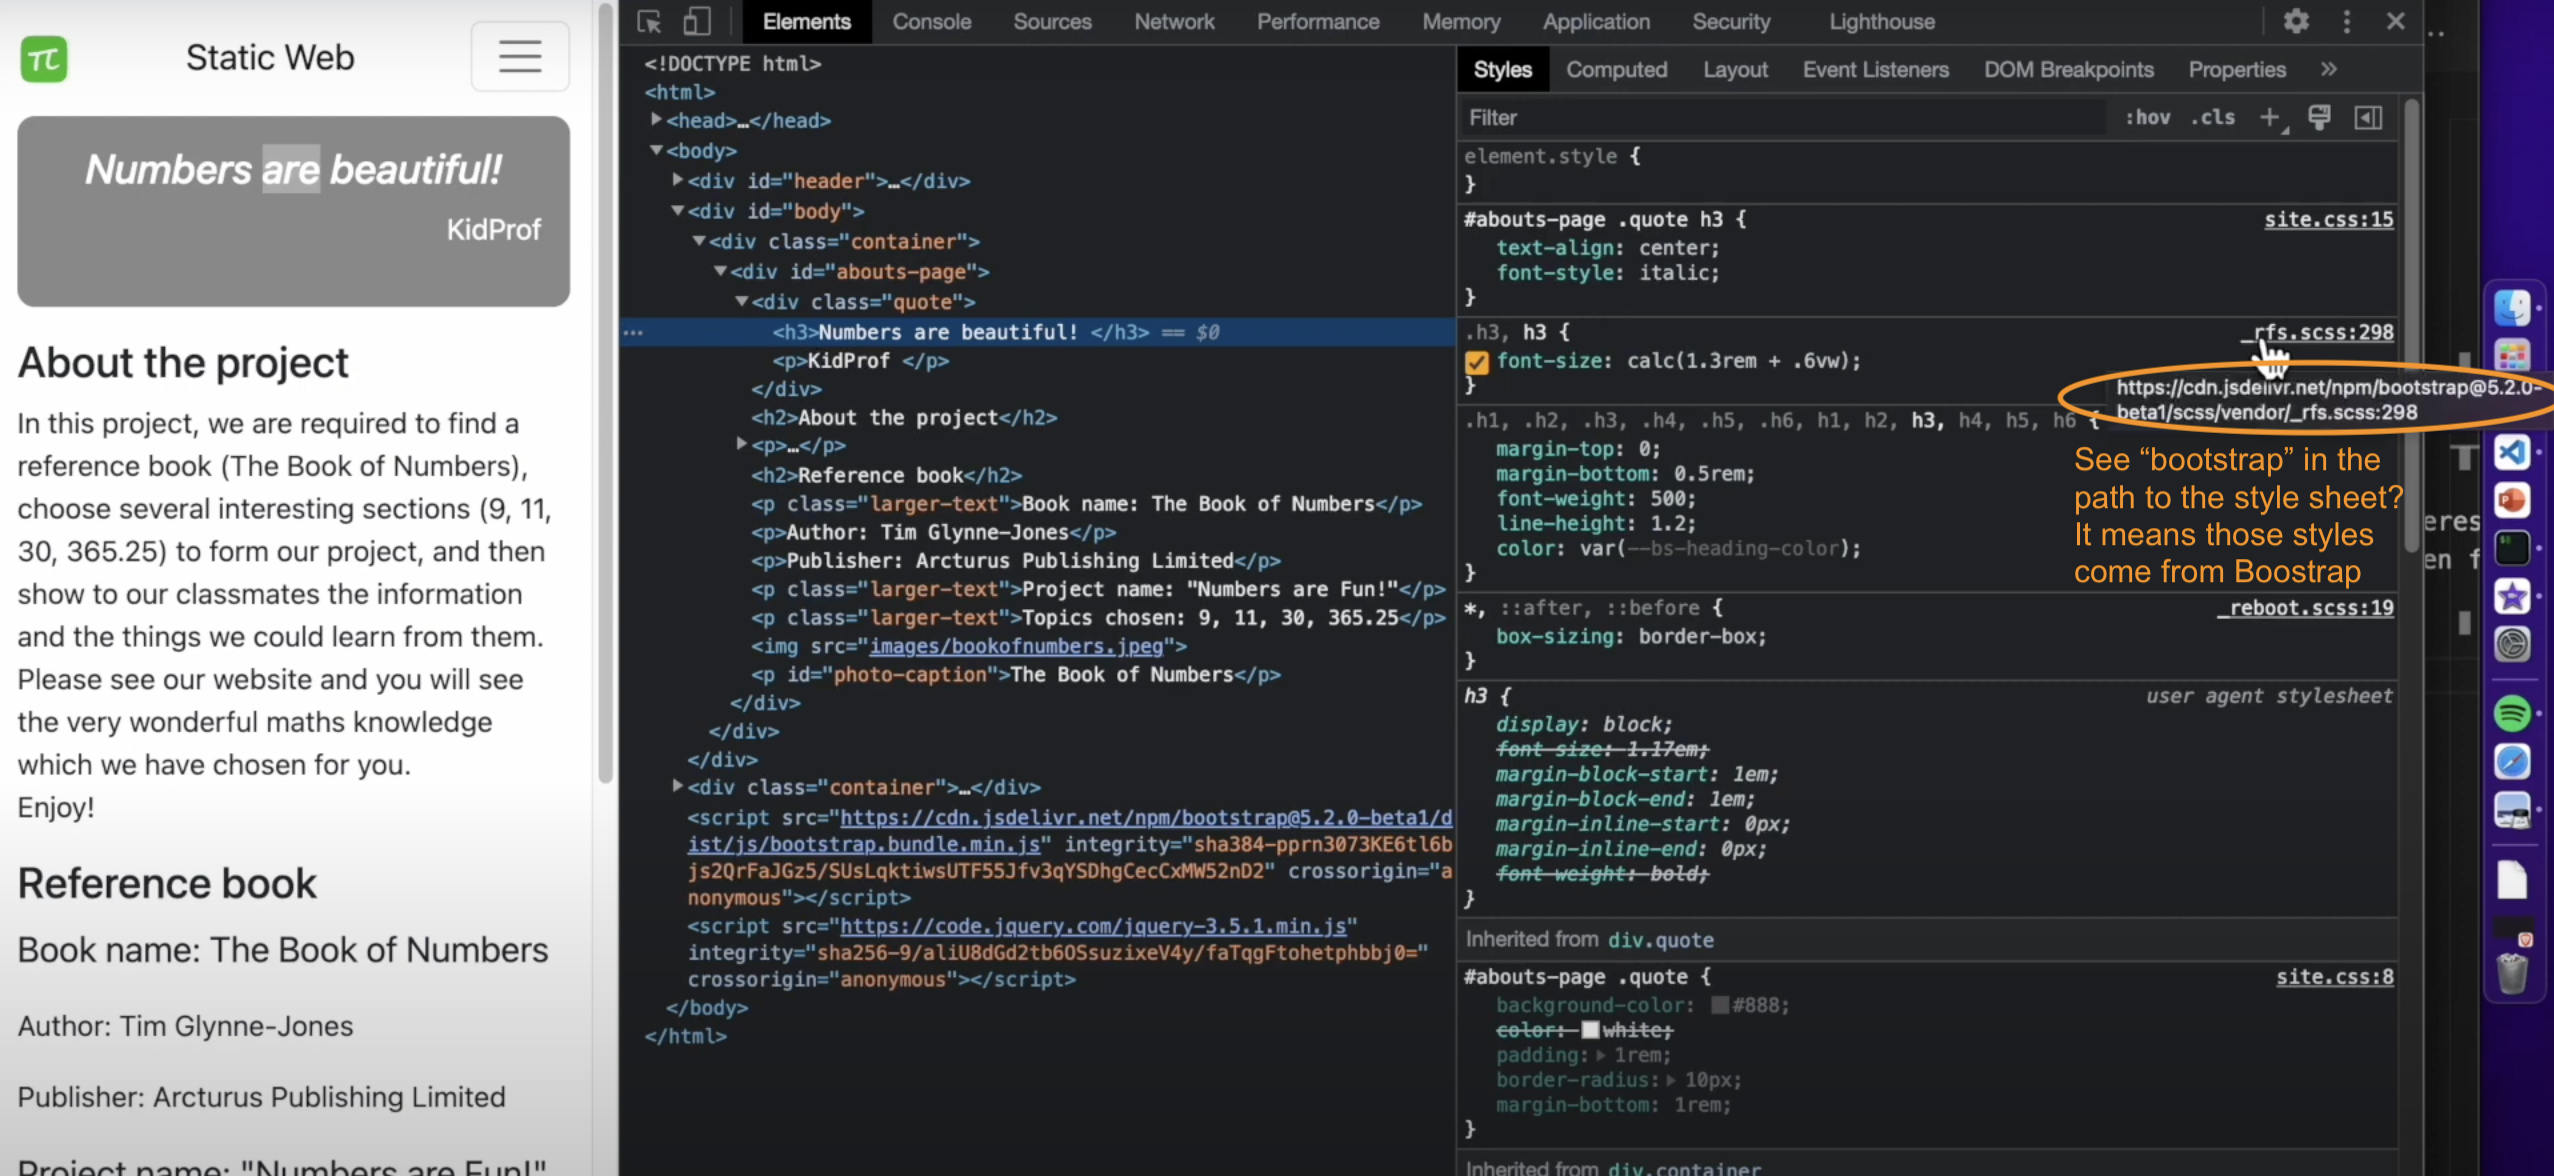
\includegraphics[width=15cm]{images/chn7-bootstrap-default-styles.png}
\caption{Proof that the default styles come from  Bootstrap}
\end{figure}

This fact concludes that Bootstrap makes the website prettier already without us doing anything.

\subsection*{Containers}
\label{sec:container}

\texttt{.container} is a class provided by Bootstrap that makes sure the contents does not go past the left border and the right border, so that the contents are aligned and look more consistent. 

That is why we included that under \texttt{block content}, and wrap everything inside it for every page all along.

\section{Helper classes}
\label{sec:classshorthands}

Bootstrap provides a number of styling short hands through helper classes.

For example, in \cref{sec:grid} we used these code to set the width of the image to be as wide as the allocated columns.

\begin{lstlisting}[language=pug]
img#bookofnumbers(src="images/bookofnumbers.jpg")
\end{lstlisting}

\begin{lstlisting}[language=pug]
#bookofnumbers{
    width: 100%;
}
\end{lstlisting}

Bootstrap allows us to use their helper class \texttt{.w-100} to do so instead. Using helper classes means that we do not need to assign IDs to the element we want to style, and also do not need to edit the Less file at all. 

\begin{lstlisting}[language=pug]
img.w-100(src="images/bookofnumbers.jpg")
\end{lstlisting}

\begin{lstlisting}[language=pug]
// No need to add anything in the Less file
\end{lstlisting}

However, the downside of the helper classes is that they are quite restrictive. So in practice we use a combination of the traditional way introduced all throughout \cref{sec:styling} and helper classes while doing styling.

\begin{table}[H]
    \centering
    \caption{Table of common helper classes}
    \vspace{6mm}
    \begin{tabular}{|m{8em}|m{27em}|}
        \hline
        \textbf{Helper class} & 
        Description/ Equivalent CSS
        \\ \hline \hline
        
        \texttt{.w-100} &
        \texttt{width: 100\%;}
        \\ \hline
        
        \texttt{.d-none} &
        \texttt{display: none;}
        \\ \hline
        
        \texttt{.d-block} &
        \texttt{display: block;}
        \\ \hline
        
        \texttt{.text-center} &
        \texttt{text-align: center;}
        \\ \hline

        \texttt{.text-primary} &
        Set the text to a blue colour. Refer to \href{https://getbootstrap.com/docs/5.2/utilities/colors/}{the documentation} for other colours.\tablefootnote{Documentation: \url{https://getbootstrap.com/docs/5.2/utilities/colors/}  (V5.2)}
        \\ \hline

        \makecell[lb]{
            \texttt{.mt-1} \\
            \texttt{.ps-2} \\
            \texttt{.pe-3} \\
            \texttt{.mx-4} \\
            \texttt{.p-5}
        } & 
        \makecell[lb]{
            \texttt{margin-top: 0.25rem} \\
            \texttt{padding-left: 0.5rem} (\texttt{s} for start)\\
            \texttt{padding-right: 1rem} (\texttt{e} for end)\\
            \texttt{margin: 0 1.5rem 0 1.5rem} (\texttt{x} for x-axis)\\
            \texttt{padding: 3rem 3rem 3rem 3rem;}
            (All sides)
        } 
        \\ \hline
        
    \end{tabular}
\end{table}

More on margins and paddings helper classes: 
\texttt{m} for margin, \texttt{p} for padding, \texttt{1} to \texttt{5} indicates the amount of spacing needed. Refer to 
\href{https://getbootstrap.com/docs/5.2/utilities/spacing/#margin-and-padding}{the documentation}
\footnote{Documentation: \url{https://getbootstrap.com/docs/5.2/utilities/spacing/\#margin-and-padding}  (V5.2)} for more options available by Bootstrap.


\section{Components}
\label{sec:components}

In the following two sections, we would go over how to use two of the Bootstrap components in detail. The idea is after we have done so, you would be able to understand the general way of using all Boostrap components by reading the documentation on your own.

What I would do first is to check out all the components in the list and find out which component suits the best for the look I envisioned. (Or if there is none that might help then we can write our own styles like in \cref{sec:styling})

\subsection{Carousel}
\label{sec:carousels}

\textit{Covered in \href{https://www.youtube.com/watch?v=kNHgf6cjdBQ&list=PLjGmdnqrOKuYXiu7lgG5HW71jPEUd1XCm&index=10}{video 8 of the series}}
\vspace{6mm}

\begin{figure}[h]
\centering
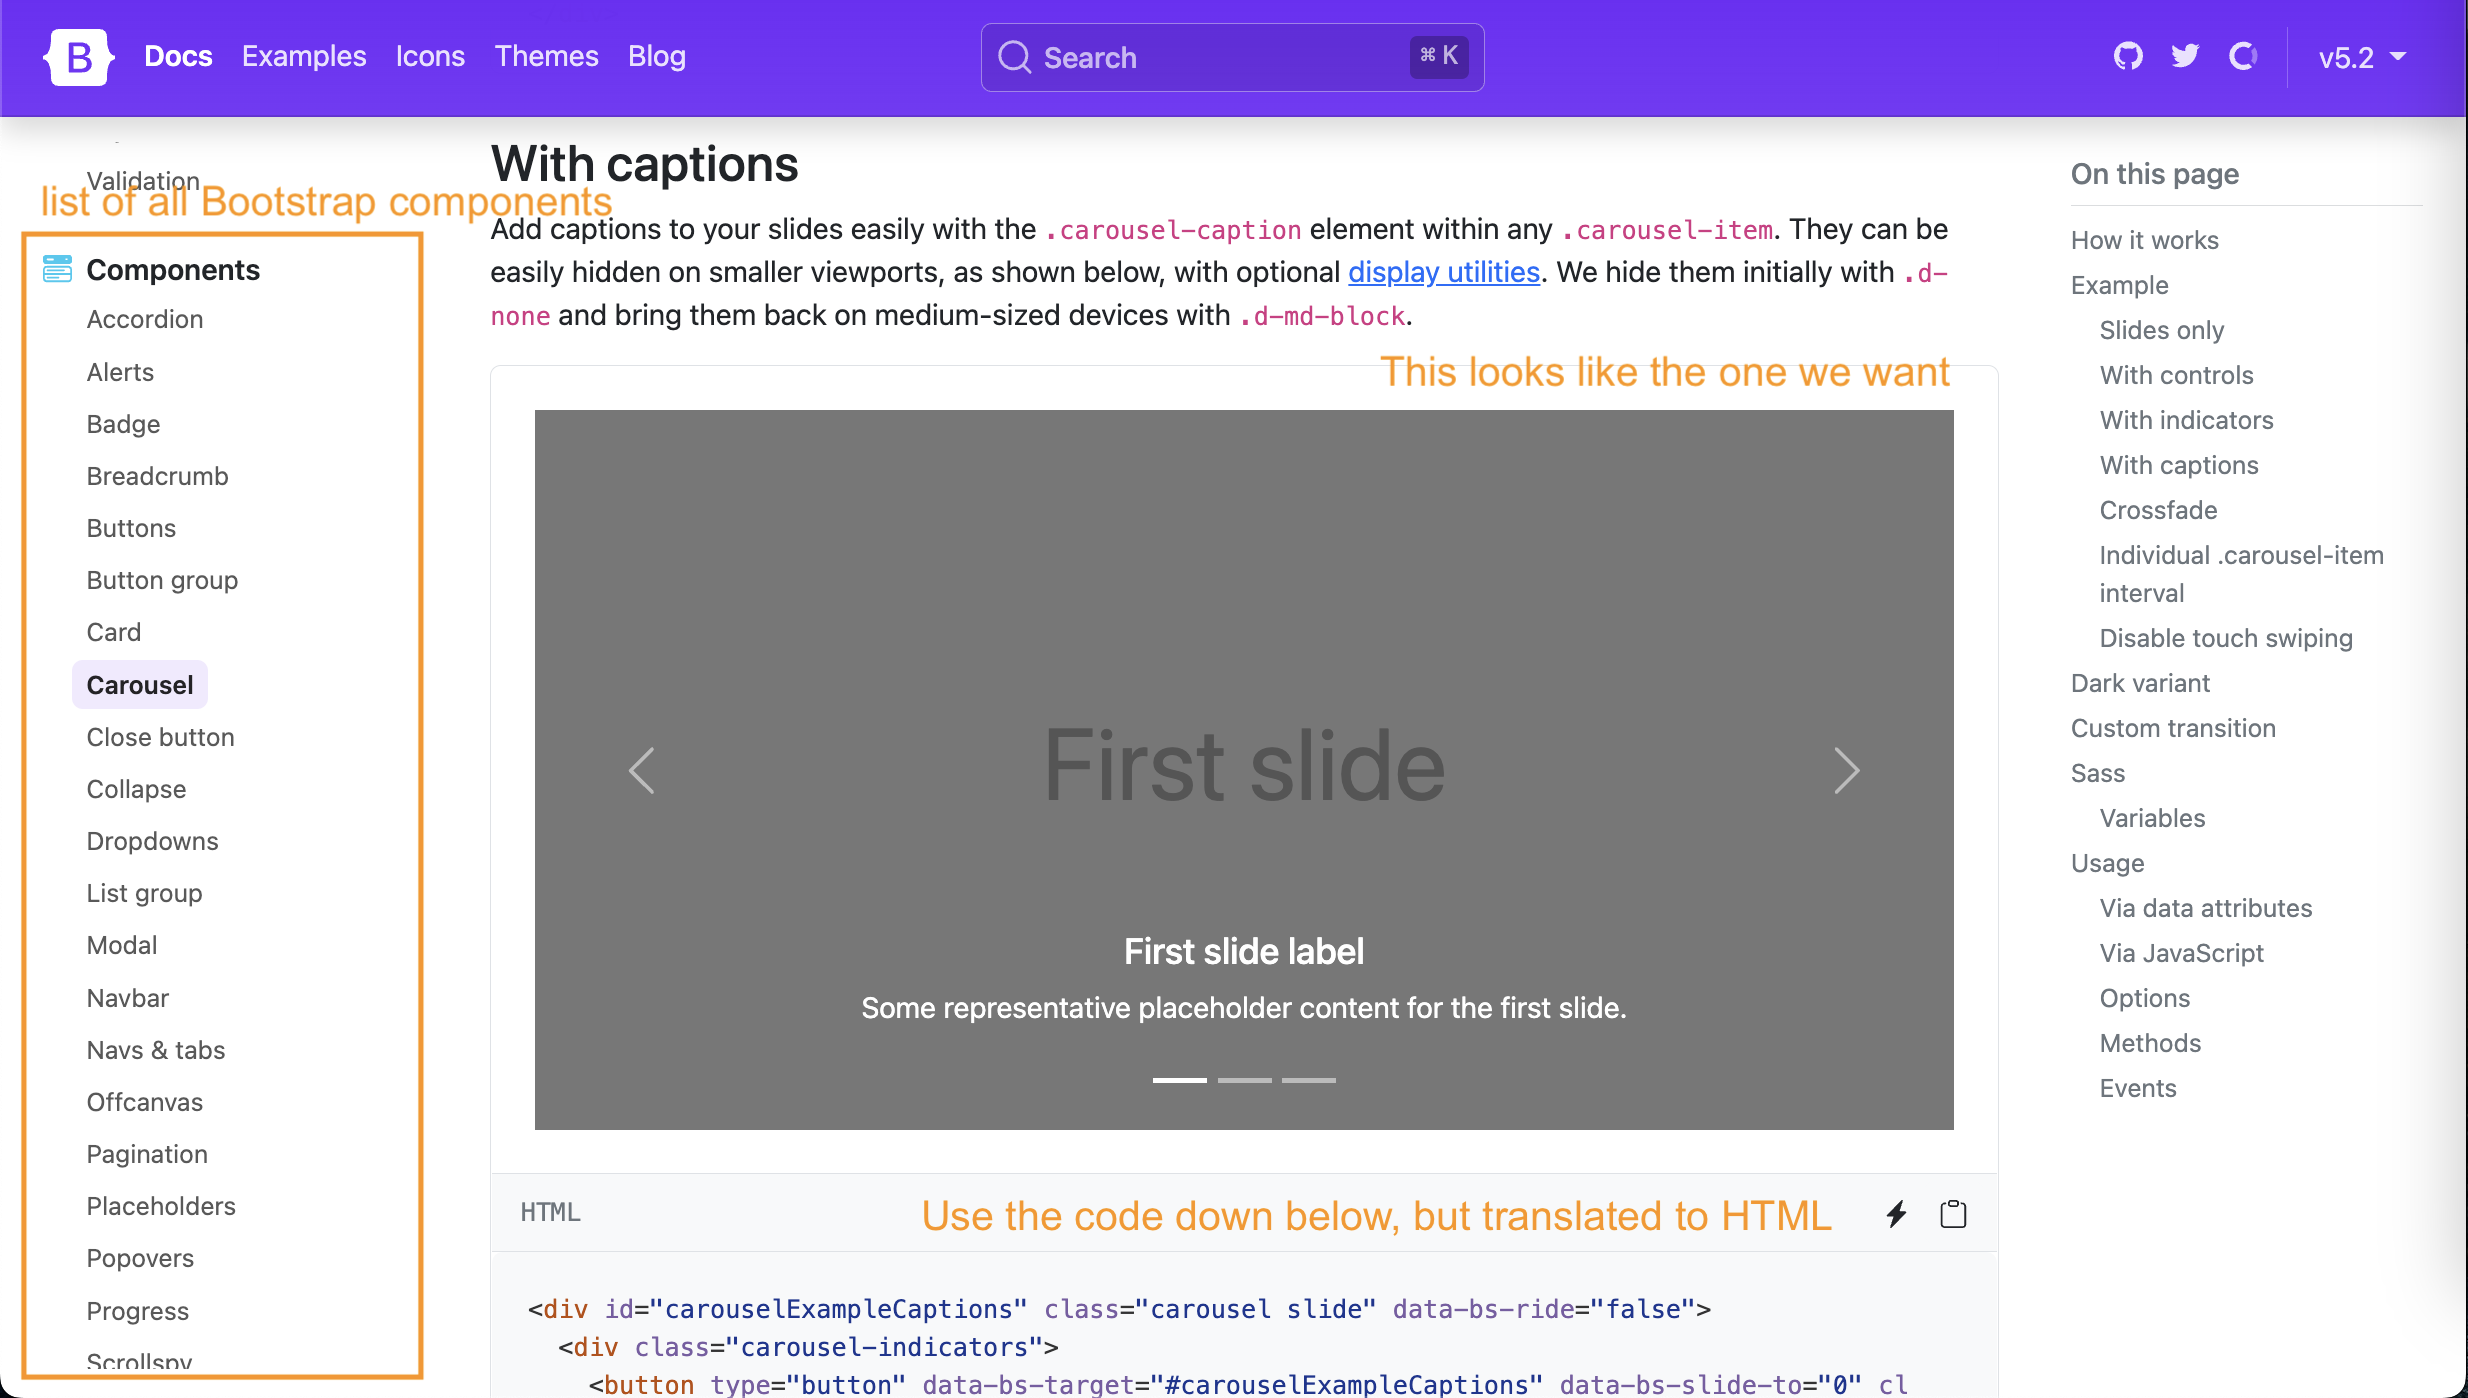
\includegraphics[width=15cm]{images/chn7-carousel-docs.png}
\caption{Bootstrap documentation}
\end{figure}

The carousel is a slideshow for cycling through a series of images, that seems quite a fit for the index page. So I go to the \href{https://getbootstrap.com/docs/5.2/components/carousel/}{documentation page of the carousel}\footnote{Link: \url{https://getbootstrap.com/docs/5.2/components/carousel/} (V5.2)}. You can find the carousel documention by searching for "carousel" in the search box, or scroll through the menu on the left of the documentation. 

Then I scroll down to the sample section of the carousel documentation and find the one that I like the most. I think the "With captions" one suit our sample web site. Then, we copy the code down below. However, the code provided is in HTML, and we need to translate them to Pug. Follow \href{https://html-to-pug.com/}{this URL}\footnote{Link: \url{https://html-to-pug.com/}} for an online translator for that. However, doing the translation by yourself is a good exercise to further familiarise yourself with the Pug syntax. 

If you are having trouble with the translation, you can checkout \href{https://www.youtube.com/watch?v=kNHgf6cjdBQ&list=PLjGmdnqrOKuYXiu7lgG5HW71jPEUd1XCm&index=10}{my video and follow step 
 by step}\footnote{Link: \url{https://www.youtube.com/watch?v=kNHgf6cjdBQ&list=PLjGmdnqrOKuYXiu7lgG5HW71jPEUd1XCm&index=10}}. Below is the basic structure of the code for easy understanding. You can view the full version on my \href{https://github.com/KidProf/numbersarefun-sample-temp/blob/main/app/templates/views/index.pug}{sample GitHub repository}\footnote{Link: \url{https://github.com/KidProf/numbersarefun-sample-temp/blob/main/app/templates/views/index.pug}}.

\begin{lstlisting}[language=pug]
.container: #myCarousel.carousel.slide.mb-4(data-bs-ride="carousel")
    .carousel-indicators
        button.active(...)
        button(...)
        button(...)
    .carousel-inner
        .carousel-item.active
            img.d-block.w-100(src="images/carousel0.png" alt="")
            .carousel-caption.d-none.d-md-block
                h3 ...
                h5 ...
        .carousel-item
            ...
        .carousel-item
            ...
    ...
\end{lstlisting}

I have made a few edits along the translation process. 

\begin{itemize}
    \item I renamed the ID of the carousel to \texttt{\#myCarousel}, remember to change the \texttt{data-bs-target} as well (highlighted in bold in the translated code).
    \item I am using the my own pictures\footnote{In case you are following, you can download the images from my GitHub repository: \url{https://github.com/KidProf/numbersarefun-sample-temp}} and text descriptions for the carousel.
    \item I used \texttt{h3} and \texttt{h5} tags instead of \texttt{h5} and \texttt{p} tags so that the descriptions are larger.
    \item \texttt{data-bs-ride="carousel"} is used in place for \texttt{data-bs-ride="false"}, so that the images changes automatically every few seconds.
    \item \texttt{.mb-4} is added for some space between the carousel and the cards that we are going to create in the next session. (\texttt{.mb-4} refers to some margin added to the bottom of the carousel)
\end{itemize}

Also a few things I want you to take note of.

\begin{itemize}
    \item Note the use of \texttt{.d-none.d-md-block}, it means the text description is hidden when the screen size is \texttt{xs} and \texttt{sm}, while it is shown when the screen size is \texttt{md} or larger. (Feel free to experiment with it)
    
    \item Only elements with class \texttt{.active} are shown initially. Then, the code in Bootstrap would alternate the \texttt{.active} class when switching between images. (You can open the browser developer tools to see it happening)

    \item Note the use of \texttt{:} in the first line, it is Pug.js syntax to save some indentation. For example, the following two code snippets are equivalent.

\begin{lstlisting}[language=pug]
#id1: #id2
    #id3
    #id4
\end{lstlisting}

\begin{lstlisting}[language=pug]
#id1
    #id2
        #id3
        #id4
\end{lstlisting}
    
\end{itemize}

\begin{figure}[h]
\centering
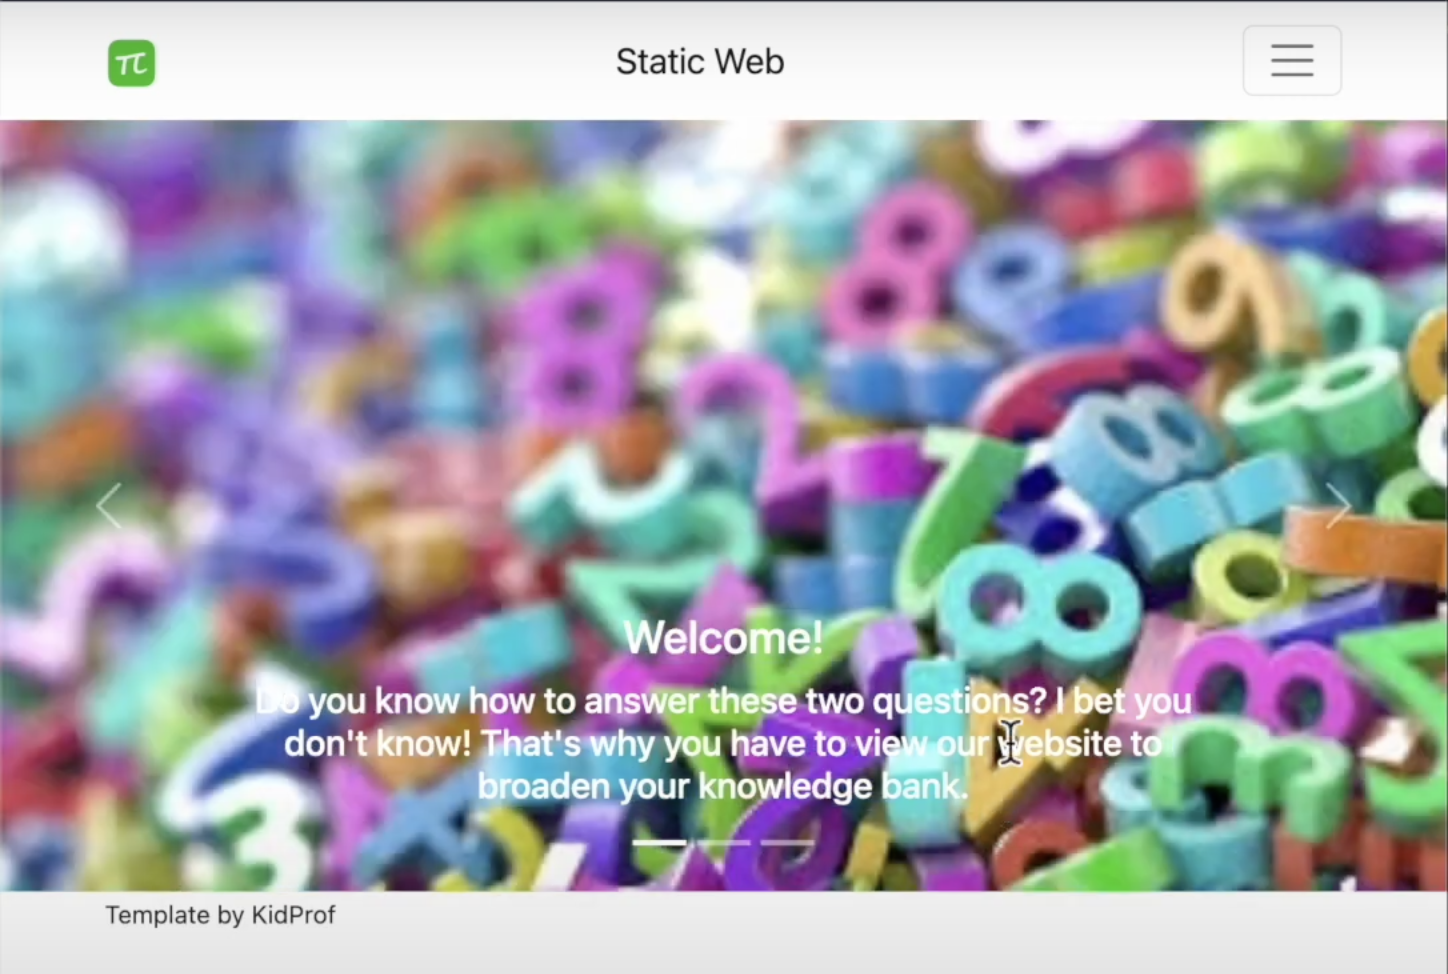
\includegraphics[width=15cm]{images/chn7-carousel-completed.png}
\caption{Completed carousel}
\end{figure}

\subsection{Card}
\label{sec:cards}

\textit{Not completed yet, as explained in \cref{sec:incompletewarning}}
% We will use Bootstrap cards\footnote{Documentation: \url{https://getbootstrap.com/docs/5.2/components/card} (V5.2)} to complete the bottom half of the index page of our sample website. Browsing through all the card examples, I would like a card with an image in the middle and a header. So my code would be a mixture of the \href{https://getbootstrap.com/docs/5.2/components/card/\#header-and-footer}{Header and Footer}\footnote{Link: \url{https://getbootstrap.com/docs/5.2/components/card/\#header-and-footer} (V5.2)} variant and the 
% \href{https://getbootstrap.com/docs/5.2/components/card/\#kitchen-sink}{Kitchen Sink}\footnote{Link: \url{https://getbootstrap.com/docs/5.2/components/card/\#kitchen-sink} (V5.2)} variant.

% \begin{lstlisting}[language=pug]
% .card
%     .card-header 
%         h3 9
%     img.card-img-top(src="images/card9.png")
%     .card-body
%         p.card-text.
%             9, may just be an ordinary number to you. ...
% \end{lstlisting}

